

\begin{figure}[h!]
\centering
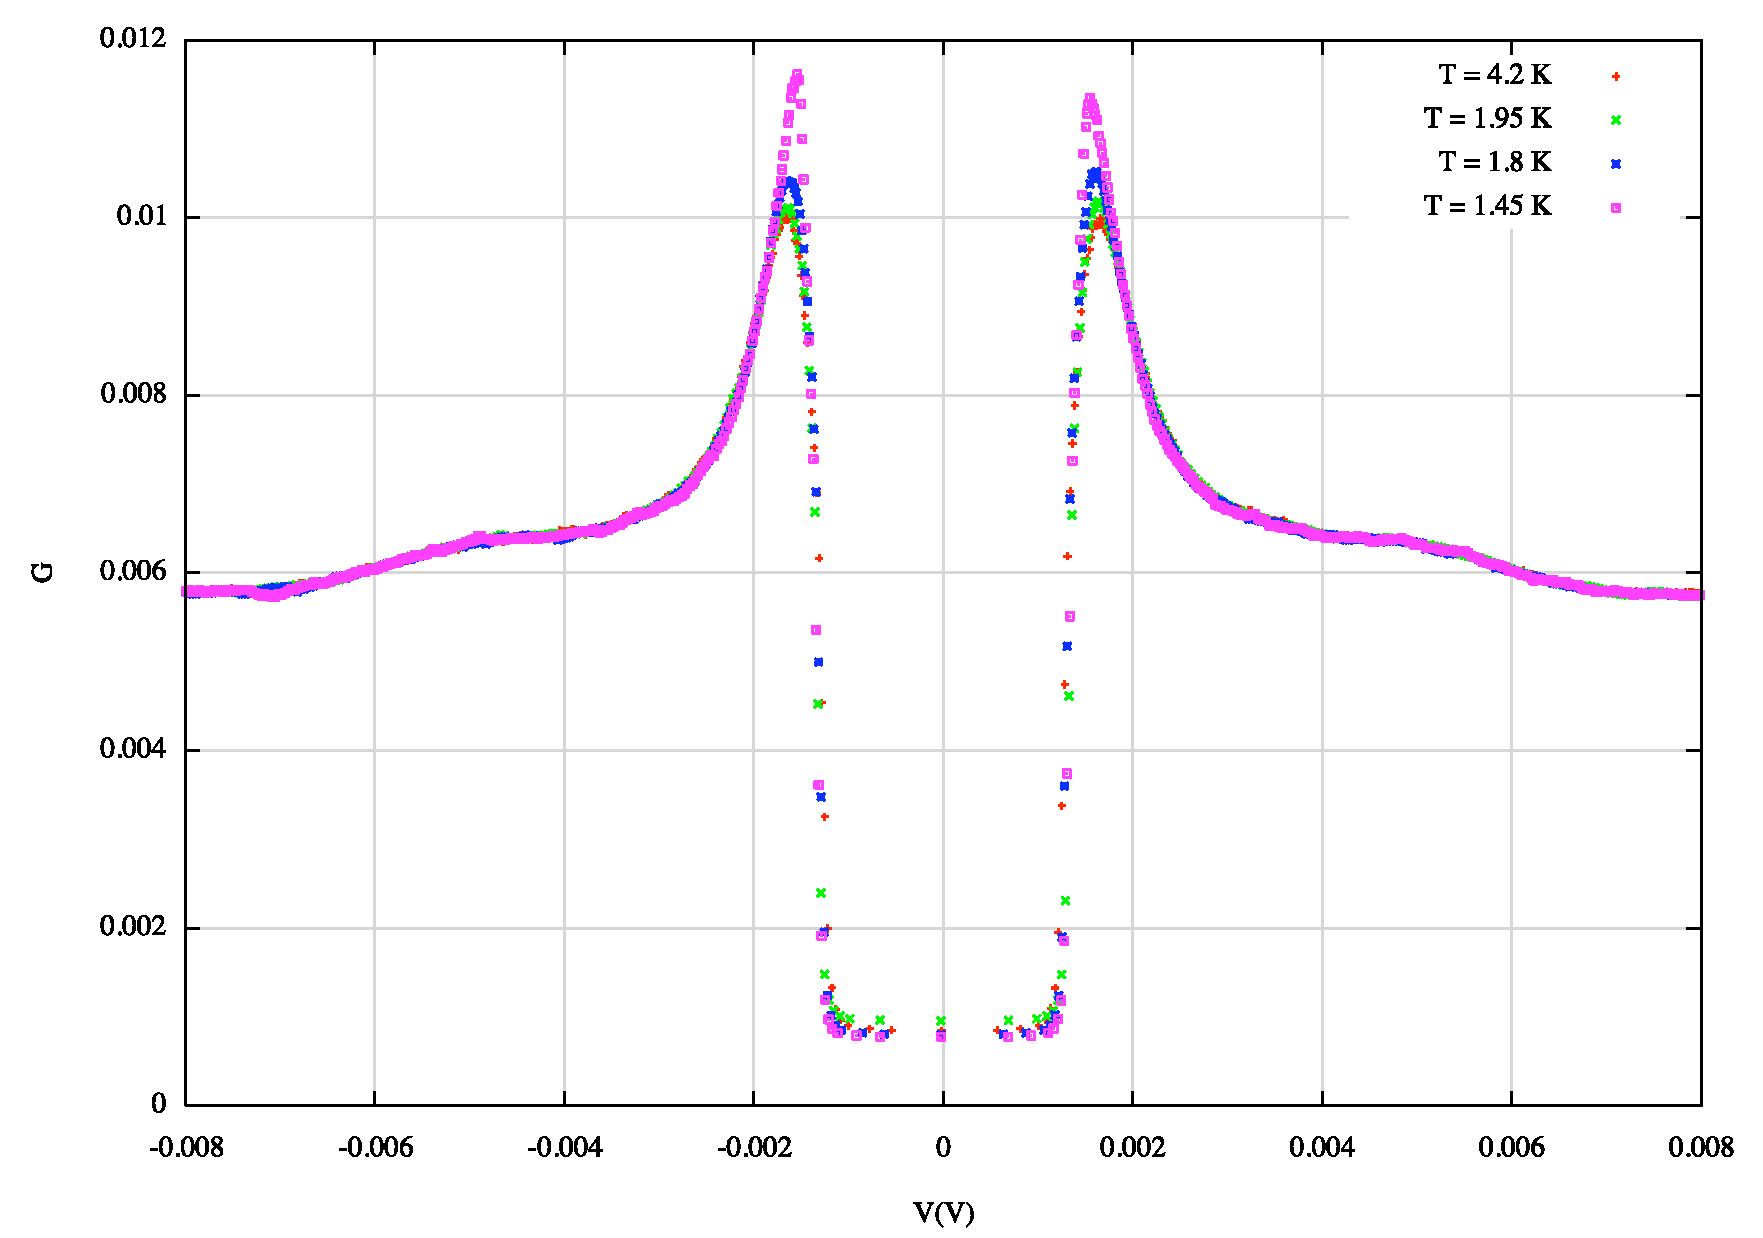
\includegraphics[width=0.45\textwidth]{gv_3-4-5-7}
\caption{Hola\label{gv_3}}
\end{figure}

\begin{figure}[h!]
\centering
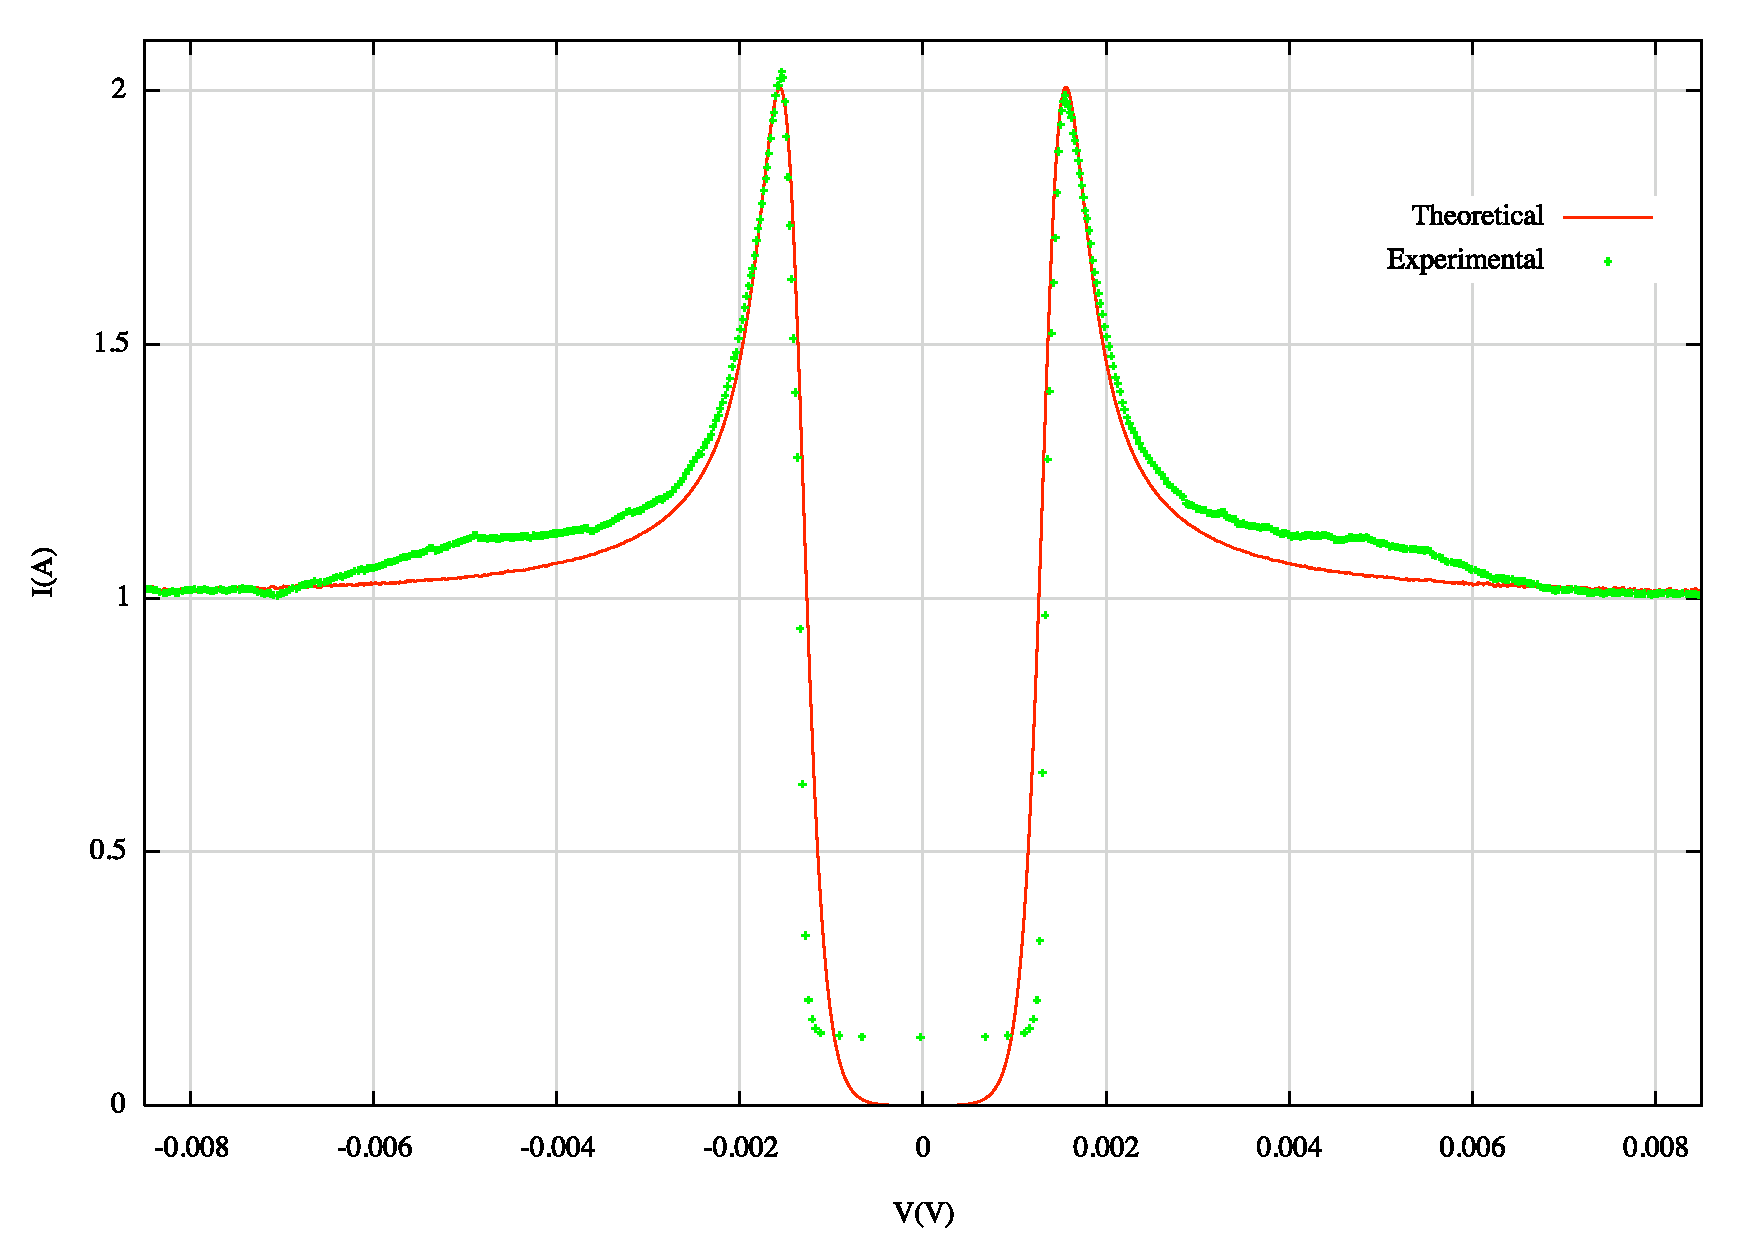
\includegraphics[width=0.45\textwidth]{gv_theo_exp_7.pdf}
\caption{Hola\label{iv_theo_exp}}
\end{figure}

\begin{figure}[h!]
\centering
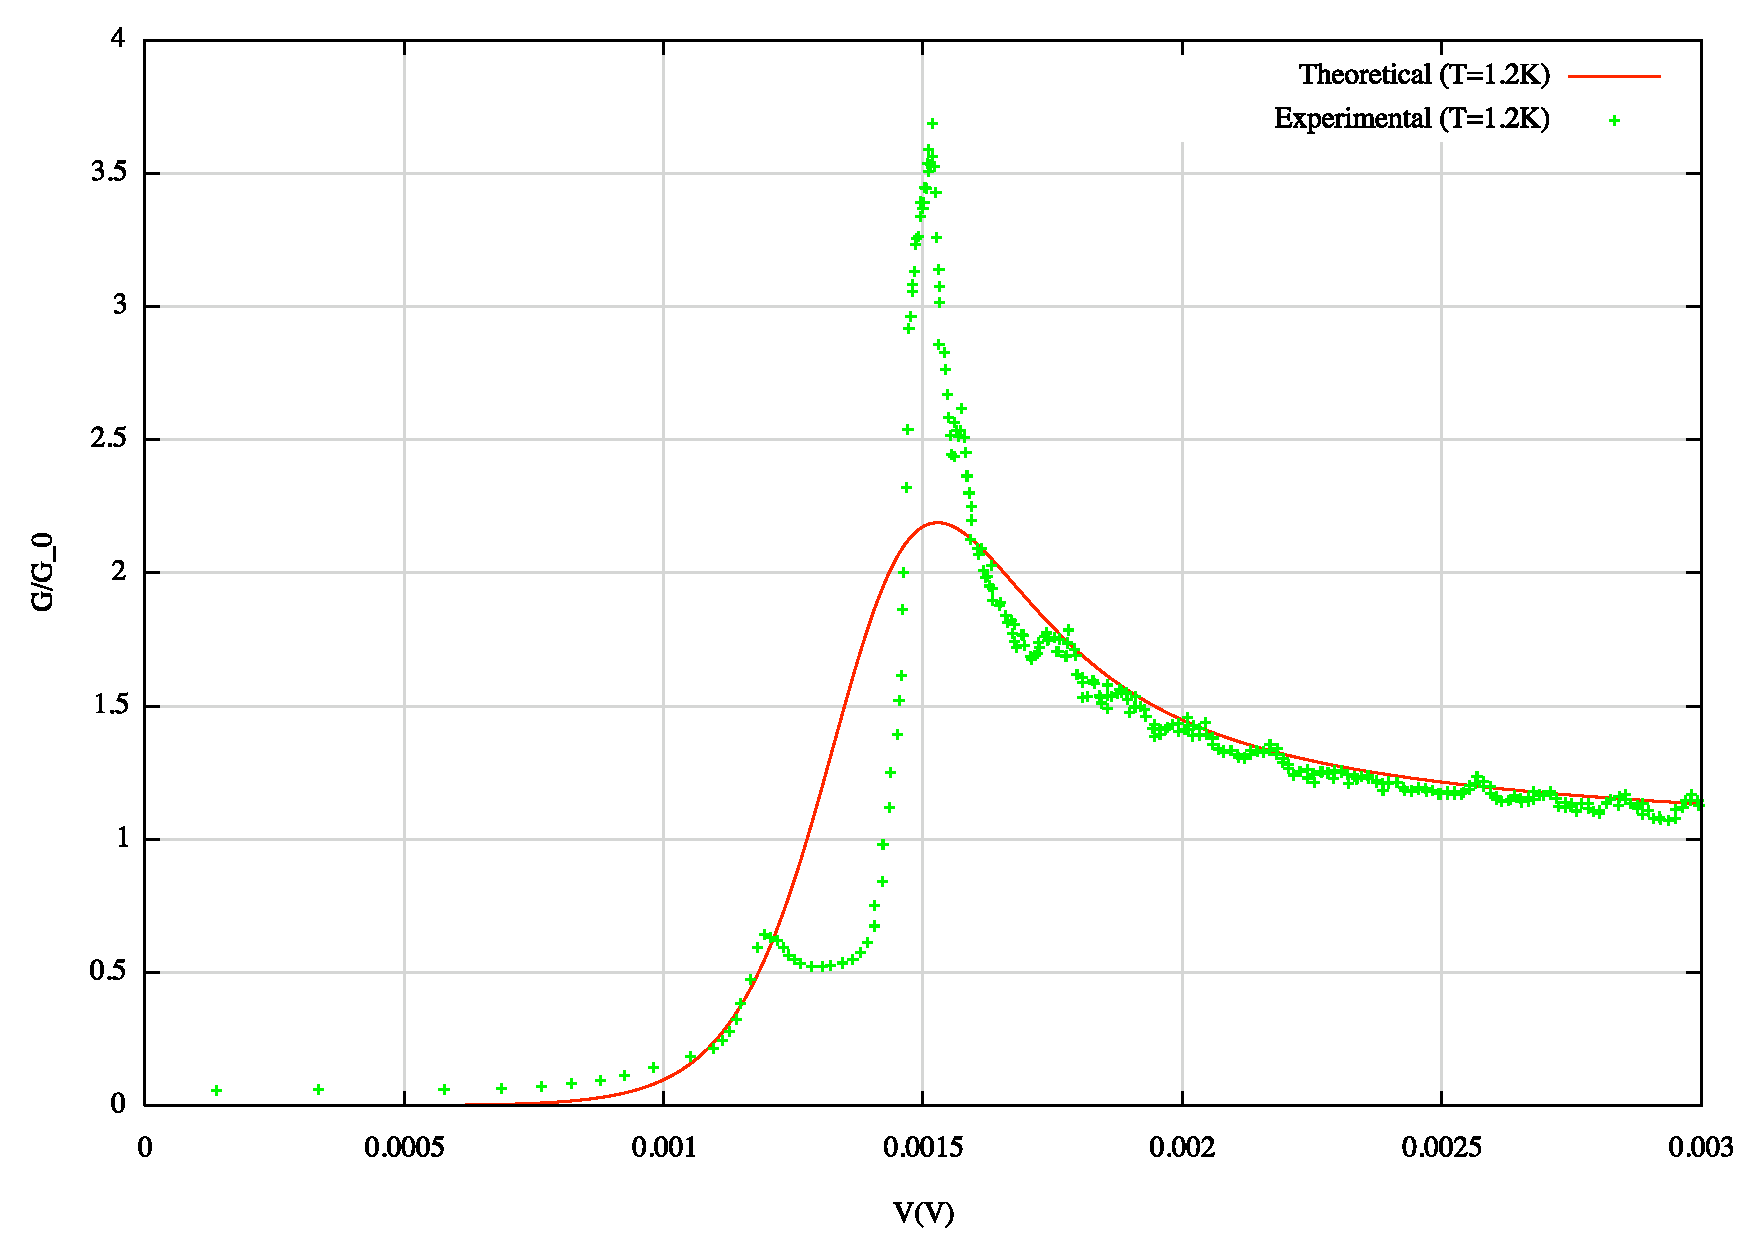
\includegraphics[width=0.45\textwidth]{gv_theo_exp_10.pdf}
\caption{Hola\label{graph3}}
\end{figure}

\begin{figure}[h!]
\centering
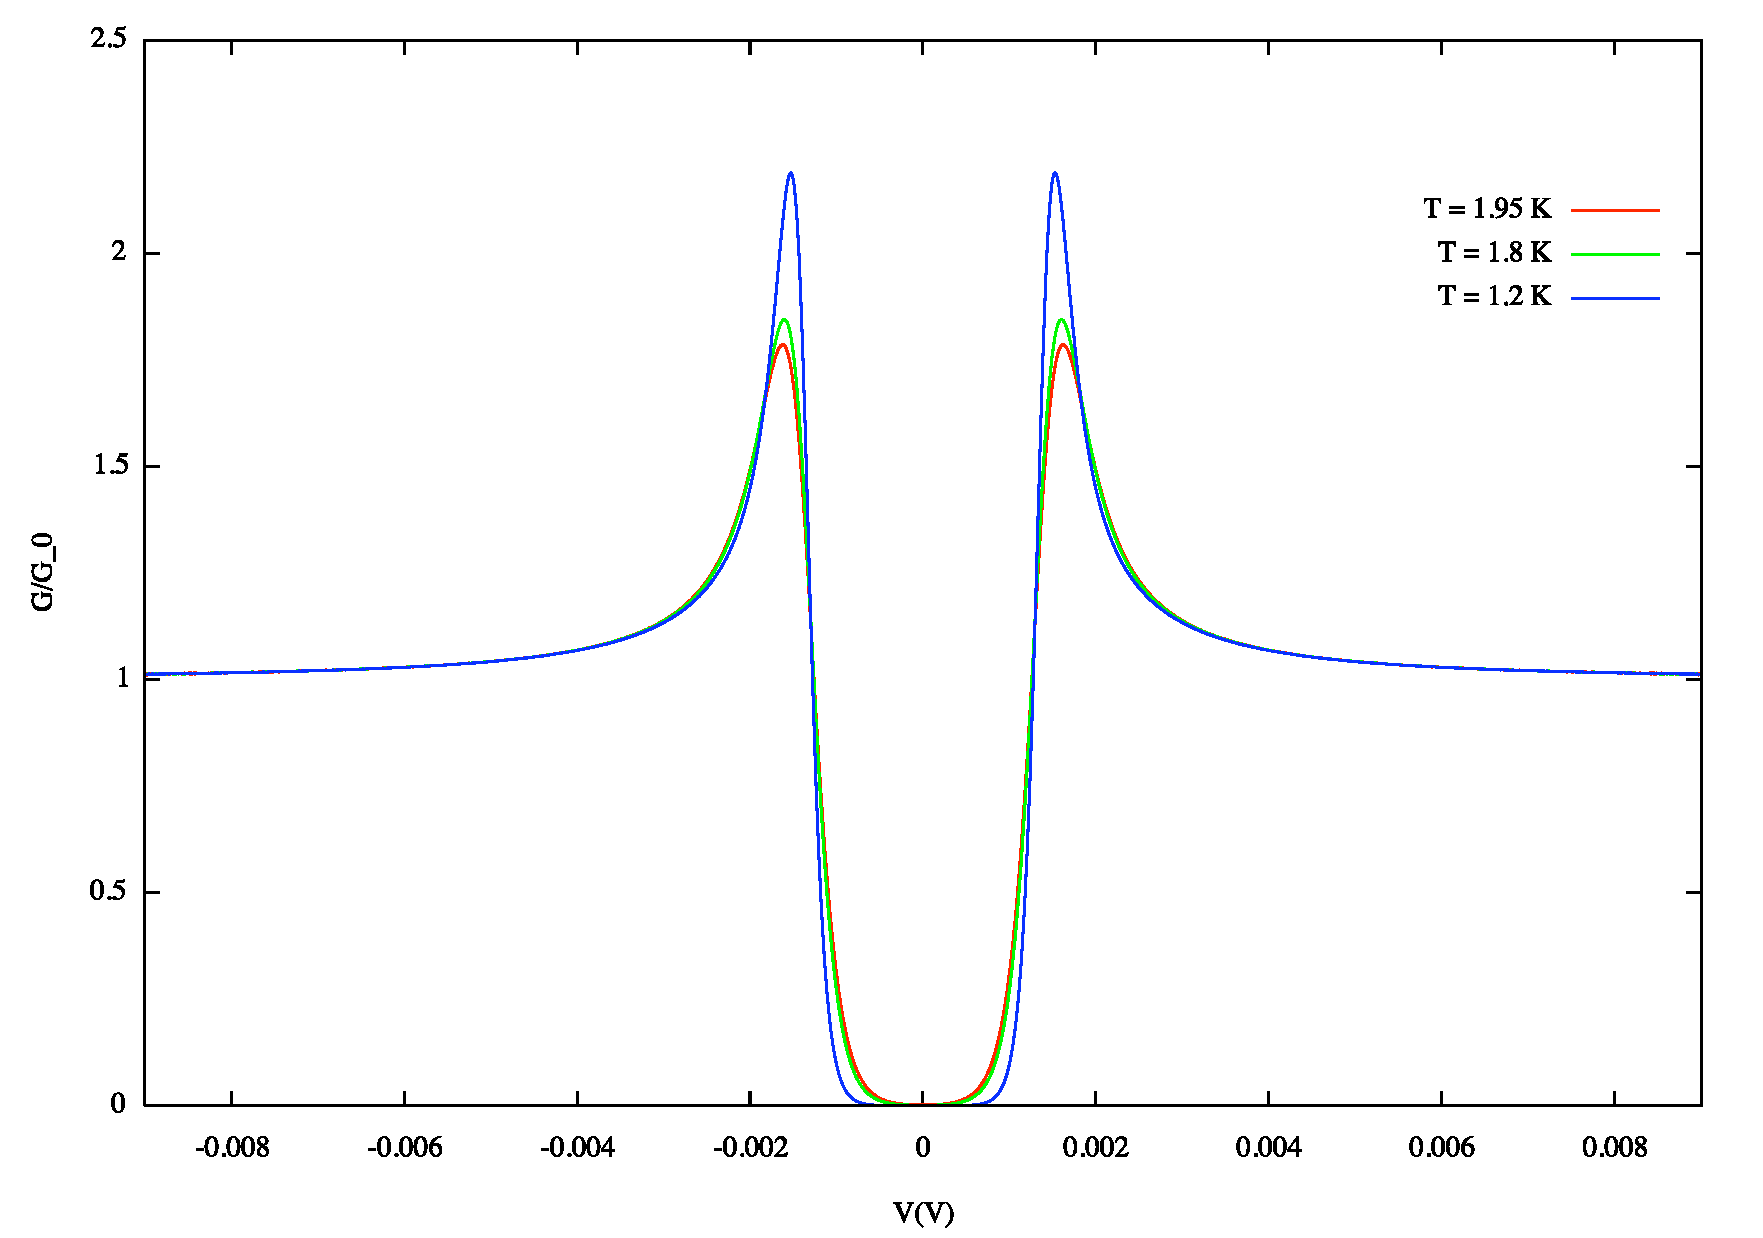
\includegraphics[width=0.45\textwidth]{gv_theoretical_4-5-10.pdf}
\caption{Hola\label{graph4}}
\end{figure}

\begin{figure}[h!]
\centering
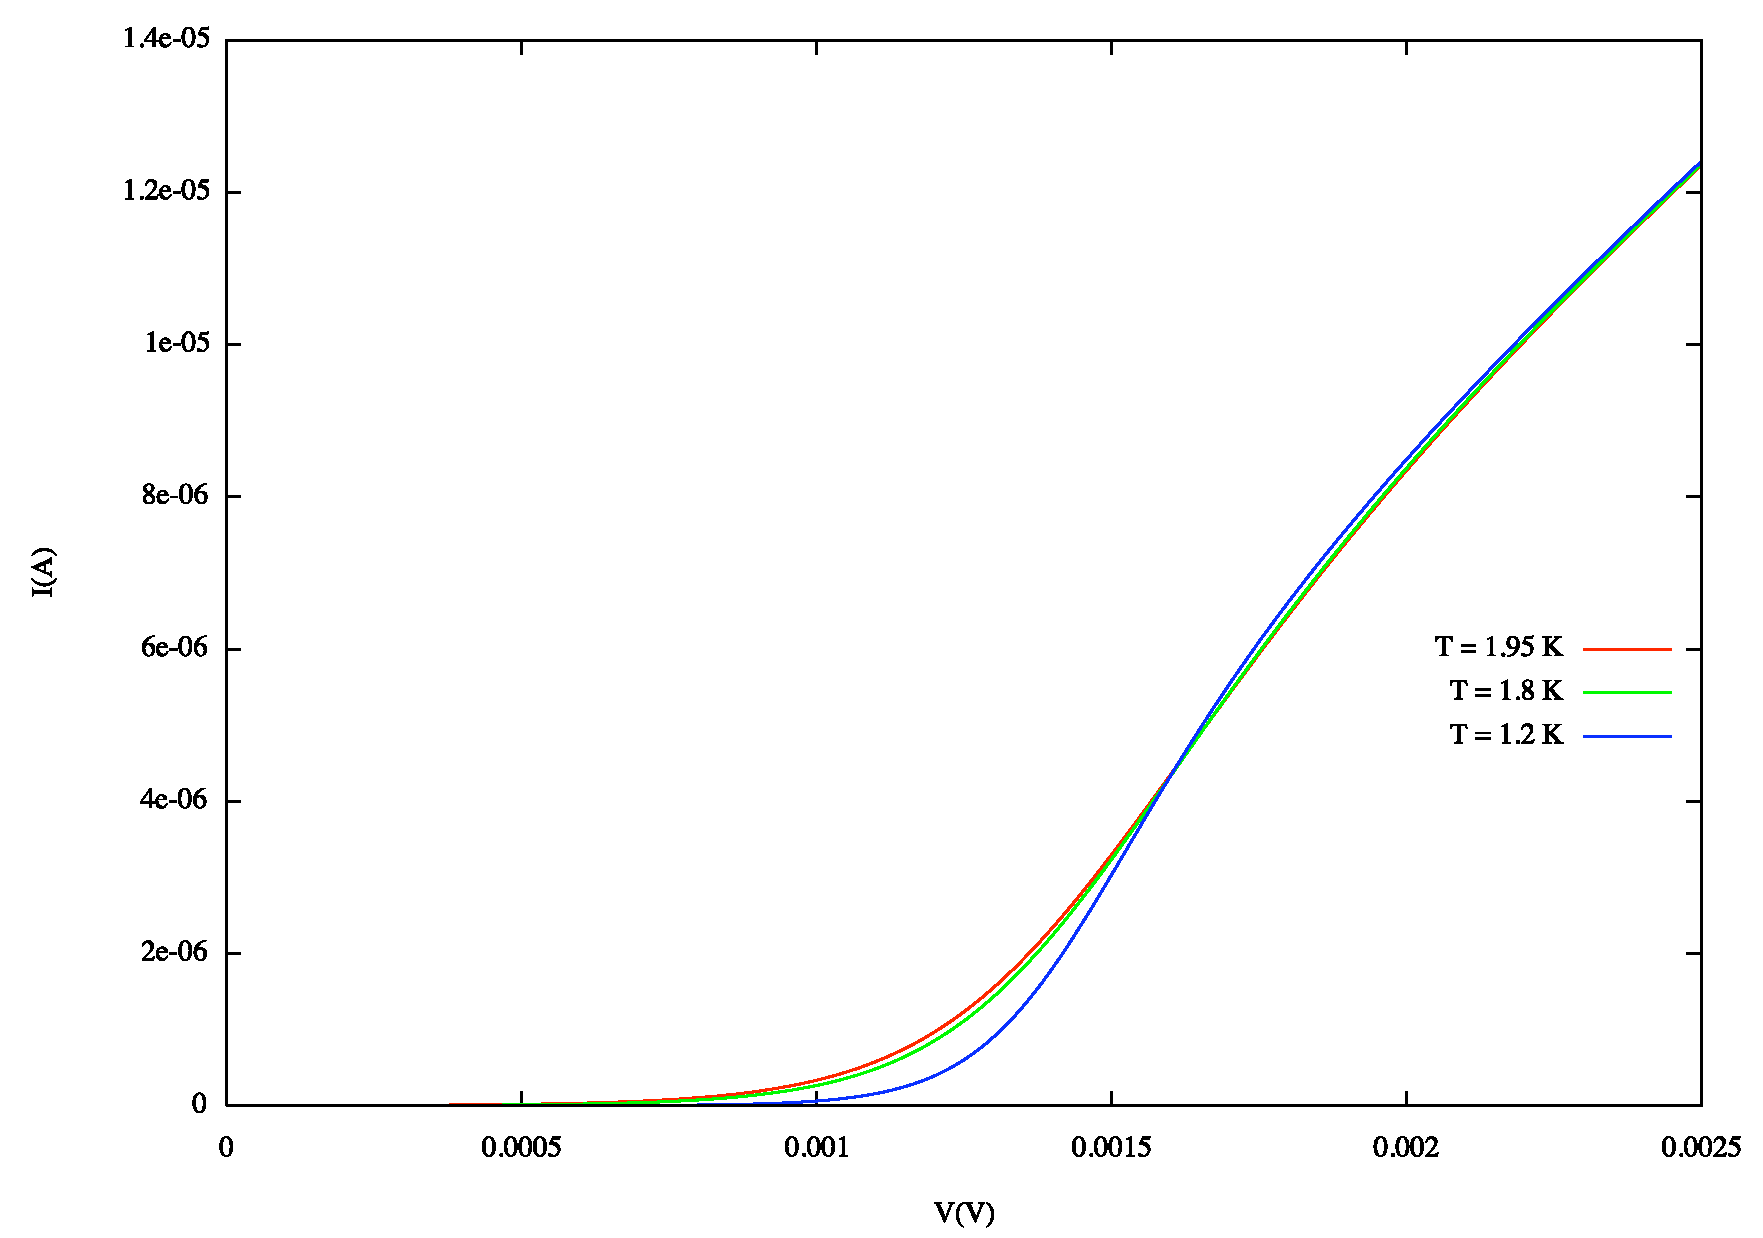
\includegraphics[width=0.45\textwidth]{iv_theoretical_4-5-10.pdf}
\caption{Hola\label{graph5}}
\end{figure}

\begin{figure}[h!]
\centering
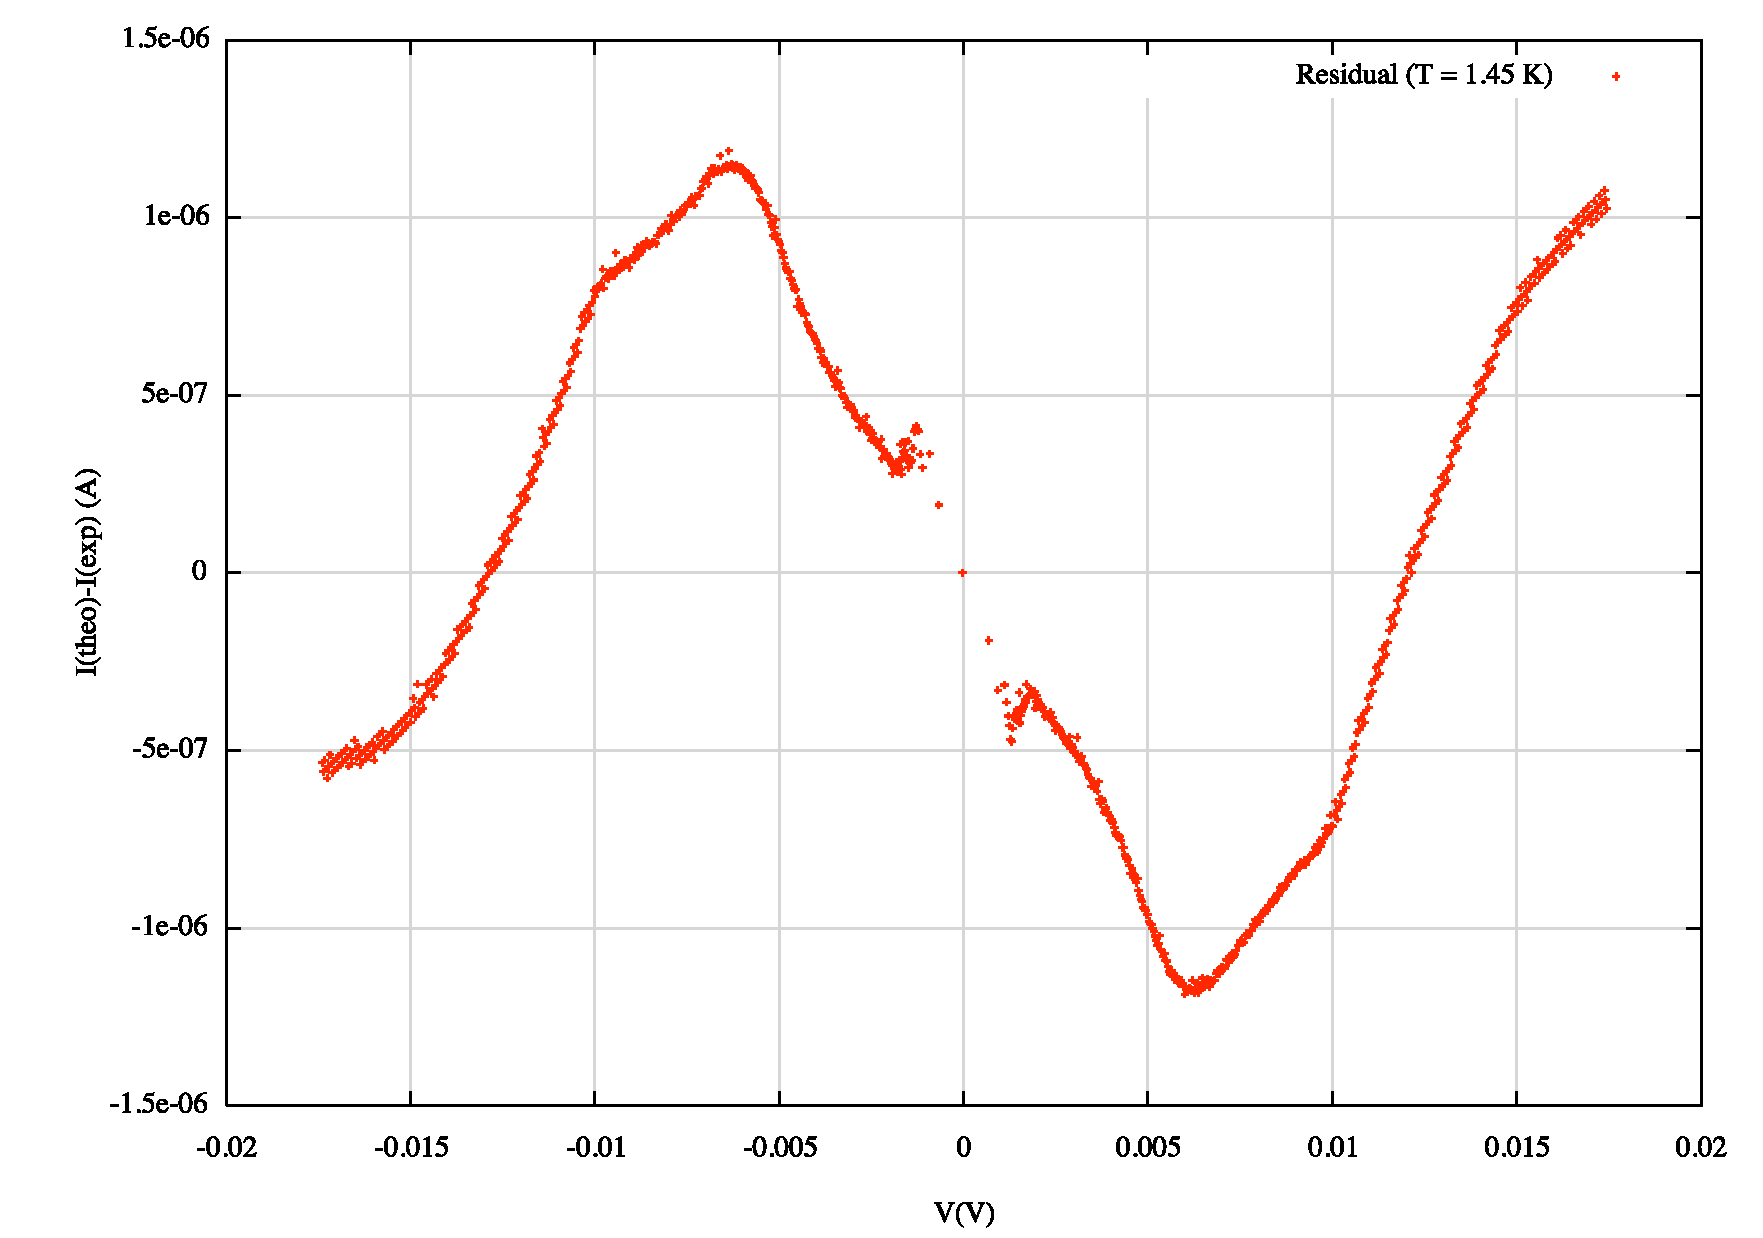
\includegraphics[width=0.45\textwidth]{residual}
\caption{Hola\label{graph5}}
\end{figure}

\begin{figure}[h!]
\centering
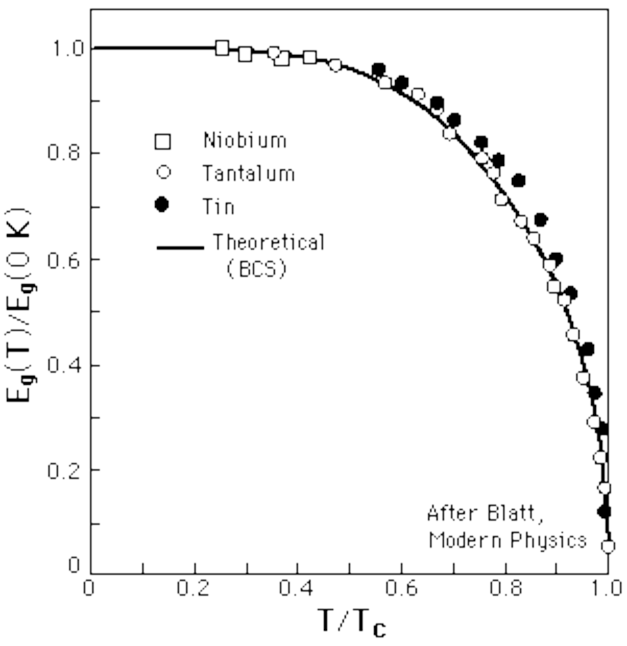
\includegraphics[width=0.45\textwidth]{bcs_gap2}
\caption{\small Reduced values of the observed energy gap as a function of the reduced temperature, after Towsend and Sutton. The solid curve is drawn for the BCS theory. \label{bcs_gap}}
\end{figure}


\begin{figure}
\centering
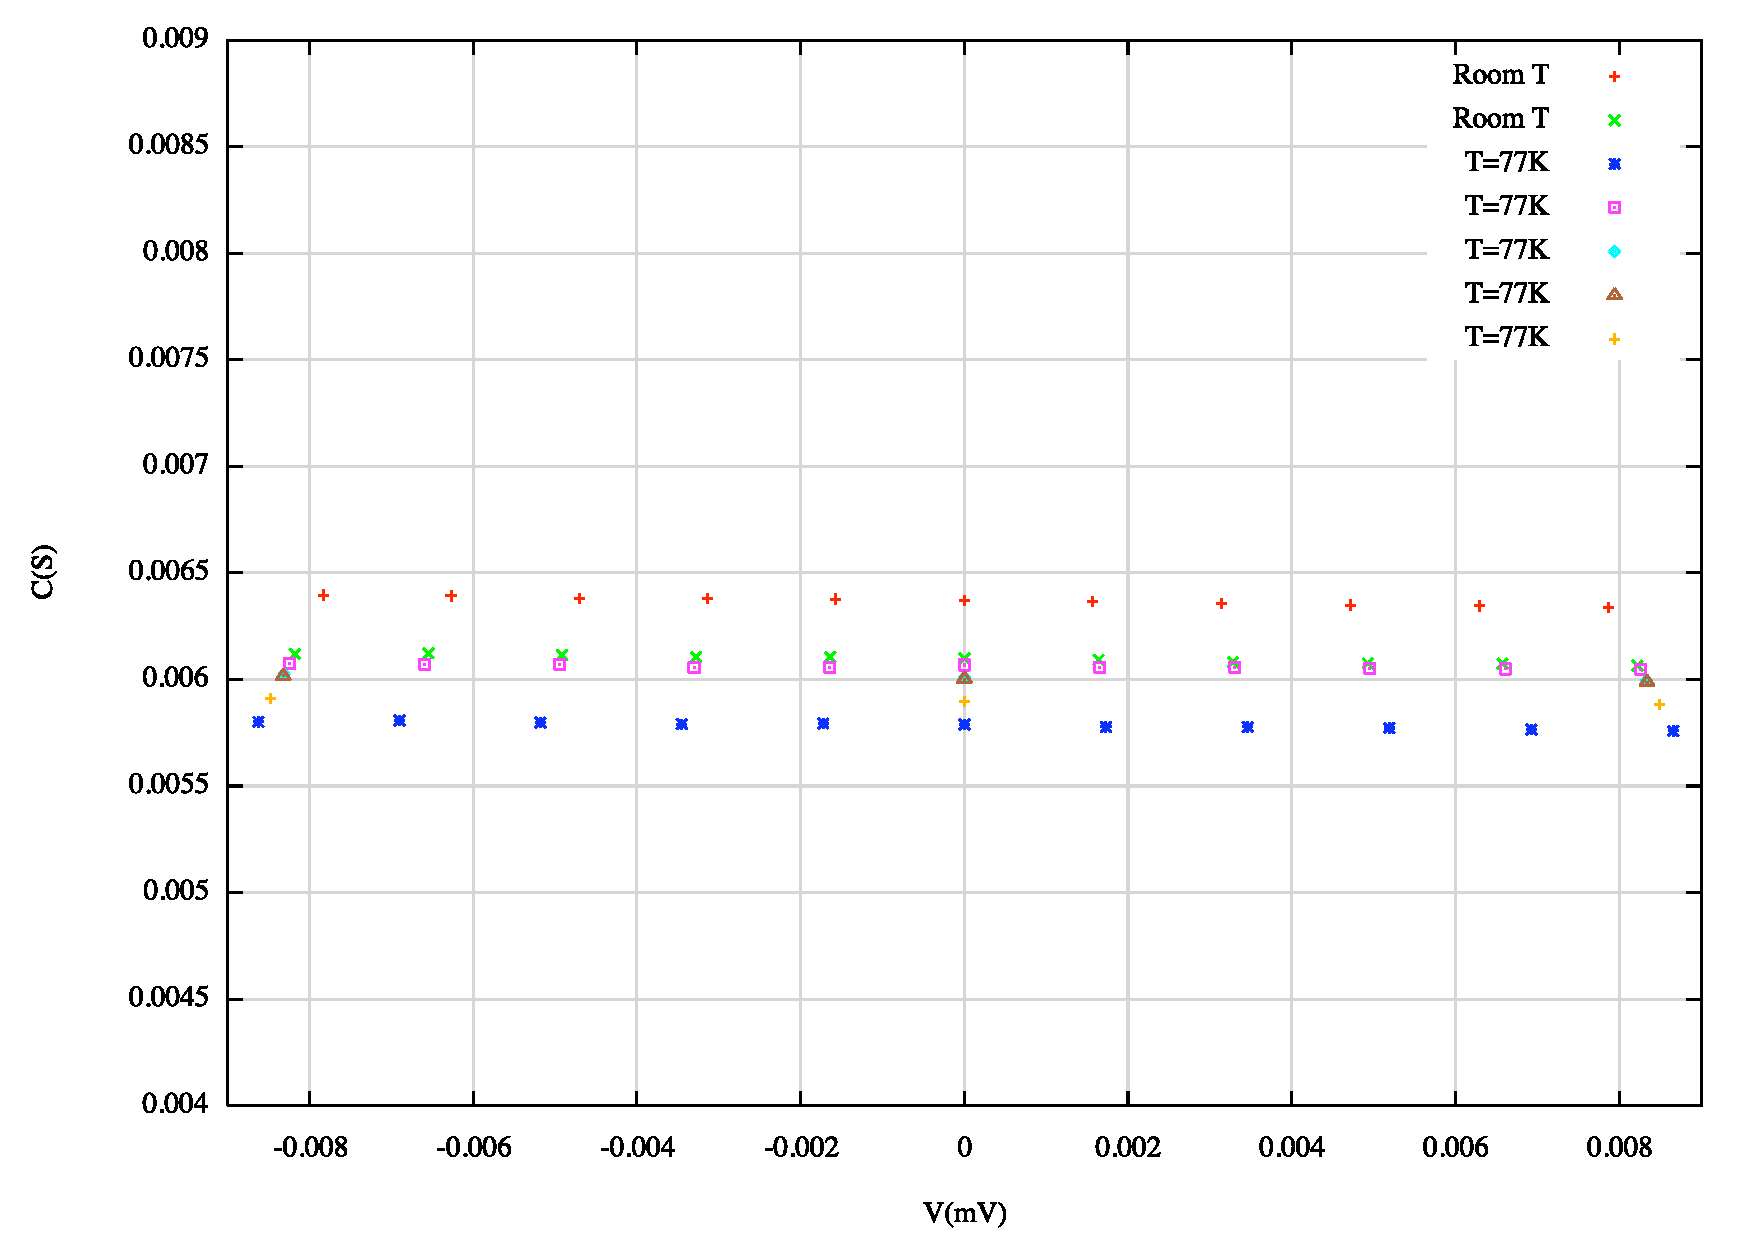
\includegraphics[width=0.45\textwidth]{conductance2}
\caption{\small Conductance curves . \label{conductance}}
\end{figure}



\subsection{Energy gap}

0.- Graphing method: smoothing (same order for theo and exp), derivation method (linear least squares, g is the slope...). Smoothig looses information...

1.- BCS does not fully describe the measured data. The density of states is different... --> Residual

2.- Might be electron-phonon scattering.

3.- Fitting by generic least squares algorithm cannot be correct.

4.- The best way: by hand. how? 
	1st : conductance by room temperature and nitrogen temperature data measurements (figure)
	2nd : T by helium vapor pressure --> manometer�?�? error??? 
	3rd : T and gap. The gap is the same for all T's because our range is small (figure). We give a sufficient large error for it (subjective...)
	4th : The temperatures are consistent

------------------

5.- Last measurement gives qualitatively different results... Possible explanation: normal-super and super-super junctions in parallel. Tc is different for films, greater than bulk Tc...



We have measured the lead's energy gap as $(1.4 \pm 0.1)meV$ below $4.2K$. The BCS theory predicts a temperature dependance, nevertheless in the range we have measured it, i.e. below the helium vaporization and above the Aluminum critical temperatures, this variation is less than the experimental error. This can be seen in fig.\ref{bcs_gap}.

The data almost agree with BCS theory. In fig.\ref{iv_theo_exp} can be seen the I-V curve, which is modified near the gap when the temperature is below the $T_c$. The experimental and theoretical data are difficult to distinguish. 

However, 



1) Symmetric?

2) Al a little bit superconducting

3) Phonons

4)  How have been made the graphs... smoothing... effects below the smoothing cannot be considered.

5) Tc for films is greater than the bulk Tc's... So at 1.2K is possible that some parts of the Al film are superconductors. In this case, we have normal-super and super-super junctions added in parallel.



